\section{Resultados e discussão}
\label{sec:resultados}

Antes de começarmos a apresentação dos resultados, análise e discussão, revisitamos e detalhamos as hipóteses propostas (Seção~\ref{sec:hipoteses}).
Em seguida discutimos o pré-processamento dos dados e alguns cuidados tomados (Seção~\ref{sec:pre-processamento}).
Finalmente, analisamos e discutimos os resultados associados a cada uma das hipóteses, em sequência (Seções~\ref{sec:resultados-hipotese-1} a \ref{sec:resultados-hipotese-3}).

\section{Hipóteses}
\label{sec:hipóteses}

As hipóteses propostas para este trabalho foram:
\begin{compactdesc}
	\item[Hipótese 1:] a aprendizagem dos alunos de DA e DS é maior nas aulas que abordam explicitamente as ferramentas (\eg, Google Analytics para DA e Python para DS), quando comparadas às aulas mais abstratas, sobre princípios, técnicas e métodos (\eg, arquitetura de dados para DA e princípio de funcionamento dos algoritmos de agrupamento para DS).

	A justificativa para essa hipótese é que as aulas sobre ferramentas guardam uma relação explícita com os requisitos das vagas de trabalho, almejadas pelos alunos.
	Cono consequência, conforme a teoria do valor da expectativa, a expectativa de que dominar esse tópico possa levar ao resultado desejado (emprego) resulta em motivação intrínseca que contribui para a aprendizagem.
	Porém, observe que essa justificativa não faz parte da hipótese proposta, haja vista que não podemos testá-la com os dados em mãos.

	\item[Hipótese 2:] a aprendizagem dos alunos de DS (não de DA) é maior nas aulas que abordam algoritmos explicitamente (\eg, ``MeanShift e DBSCAN'') do que naquelas com tópicos mais abstratos (\eg, ``o funcionamento de um neurônio'').
	A justificativa é análoga à da hipótese anterior.

	\item[Hipótese 3:] a relevância de cada tópico, o ritmo da aula e satisfação do aluno com o curso num dado instante de tempo são preditores que também afetam a aprendizagem.

	Nesse caso a justificativa baseia-se parcialmente na aprendizagem individualizada (\foreign{self-paced learning}), na qual o rítmo da aprendizagem é completamente estabelecido pelo aluno.
	Além disso, há motivações pragmáticas: a relevância, o ritmo e a satisfação são parâmetros que podem ser modificados.
	Por exemplo, a relevância pode ser abordada com base na aprendizagem significativa; o rítmo, com melhores planejamentos de aula e do curso.
	A satisfação é o parâmetro mais abstrato e abrangente, que envolve inclusive fatores institucionais como a infraestrutura, suporte ao aluno \etc.
\end{compactdesc}

\subsection{Pré-processamento}
\label{sec:pre-processamento}

A primeira etapa na análise de dados foi transformar o arquivo dos dados para o padrão \foreign{tidy-data} \cite{Wicham2014}, onde cada linha representa a resposta de um aluno para cada um dos até 4 tópicos abordados numa aula.
A Tabela~\ref{tab:dataset-raw} ilustra as primeiras linhas desse arquivo.

\begin{table}
	\centering
	\caption{As primeiras linhas do conjunto de dados utilizados neste trabalho.}
	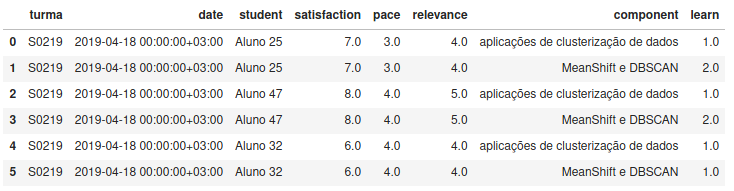
\includegraphics[width=\textwidth]{tidy-sample}
	\label{tab:dataset-raw}
\end{table}

Note que as duas primeiras linhas representam as respostas do ``Aluno 25'' ao formulário aplicado na aula de 18/abr/2019 da turma S2019. Nessa aula dois tópicos foram abordados: ``aplicações de clusterização de dados'' e ``MeanShift e DBSCAN''. No primeiro deles a aprendizagem foi de 1 unidade (última coluna) e, no segundo, de 2 unidades.

Em vista de cada formulário poder apresentar até quatro tópicos (dois neste exemplo), as informações de satisfação (\foreign{satisfaction}), ritmo (\foreign{pace}) e relevância (\foreign{relevance}) estão duplicados. Isso significa que, ao analisarmos essas variáveis, precisamos remover essas duplicidades.
Fizemos isso através de uma amostragem que selecionava, aleatoriamente, \emph{uma} linha para cada tupla (curso, turma, aula, aluno).
Por exemplo, se selecionássemos a primeira linha, certamente ignoraríamos a segunda linha.

Esse arquivo foi posteriormente transformado:
\begin{compactitem}
	\item Criamos uma coluna para identificar o curso (\foreign{course}), com valores DA ou DS, a partir da turma: aquelas que iniciam com ``A'' são de DA; as com ``S'', são DS.
	
	\item A turma foi trocada por um valor numérico sequencial arbitrário.
	
	\item As colunas de satisfação, ritmo e relevância foram normalizadas no intervalo $[0,10]$, apenas por simplicidade.

	\item Criamos a coluna \foreign{component}, que mapeia o tópico para uma hierarquia \foreign{ad-hoc} de componentes de cada curso.
	Por exemplo, o tópico ``Construção e execução de queries'' foi mapeado para o componente ``SQL/\textbf{Ferramenta}'' (DA), enquanto ``ARIMA. SARIMAX e Prophet'' foi mapeado para ``Séries temporais/\textbf{Algoritmo}'' (DS).
	O mapeamento foi feito manualmente para os 985 tópicos presentes.

	\item Criamos a coluna \foreign{tool}, variável categórica booleana, para indicar se a aula contém algum componente de ferramenta.
	Isso foi feito a partir da coluna \foreign{component}: se ela contém ``Ferramenta'', então o valor dessa variável é ``verdadeiro''; se não, é ``falso'' (veja grifos no item anterior).
	
	\item Criamos a coluna \foreign{algorithm}, variável categórica booleana, para indicar se a aula contém algum componente de algoritmo.
	Isso foi feito de maneira similar ao item anterior, também a partir da coluna \foreign{component}.
\end{compactitem}

A Tabela~\ref{fig:dataset} ilustra o conjunto de dados após esse pré-processamento e já pronto para a análise.

\begin{table}
	\centering
	\caption{O conjunto de dados, pronto para a análise.}
	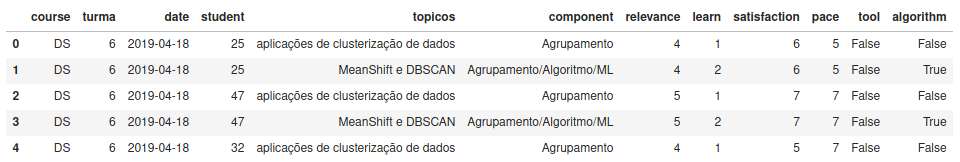
\includegraphics[width=\textwidth]{tidy-sample-2}
	\label{fig:dataset}
\end{table}
\subsection{Hipótese 1}
\label{sec:resultados-hipotese-1}

Primeiramente vamos avaliar a hipótese 1.
Nesse caso, queremos avaliar a variável dependente $a$, isto é, a aprendizagem; coluna \foreign{learn} na Tabela~\ref{fig:dataset}.
A estratégia é simples: para cada um dos cursos (DA e DS), vamos segmentar o conjunto de dados em dois sub-conjuntos, um das aulas referentes a ferramentas; o outro com o complemento deste (demais aulas).
Em seguida, aplicamos um teste de hipótese estatístico para avaliar a hipótese nula de que a média $\mu_f$ da aprendizagem da população de todas as aulas referentes a \textbf{f}erramentas é igual à média $\mu_{\neg f}$ da aprendizagem da população das demais aulas.
Ou seja,
\begin{align*}
	H_0&: \mu_f = \mu_{\neg f} \\
	H_a&: \mu_f > \mu_{\neg f}
\end{align*}

O conjunto de dados pré-processado já contém a informação de que um dado componente refere-se a uma ferramenta ou não (coluna \foreign{tool} na Figura~\ref{fig:dataset}).
Assim, podemos segregar o conjunto de dados segundo esse critério.

\begin{figure}[b]
	\centering
	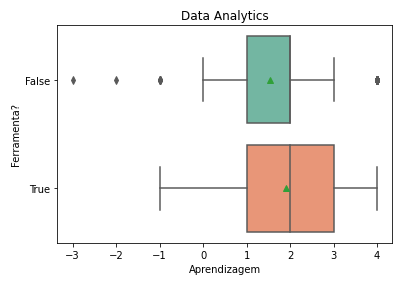
\includegraphics[width=0.45\textwidth]{da-boxplot-by-tool}\hfill
	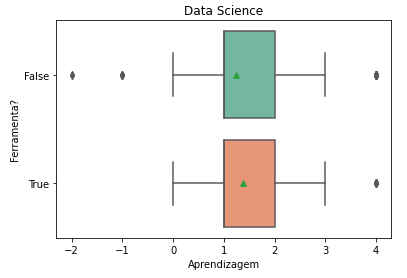
\includegraphics[width=0.45\textwidth]{ds-boxplot-by-tool}
	\caption{Distribuição da aprendizagem nos cursos de DA (esquerda) e DS (direita) para as aulas de ferramentas (\foreign{true} no eixo vertical) e as demais. Os triângulos verdes indicam a média amostral.}
	\label{fig:dist-hipotese-1}
\end{figure}

Note que a hipótese 1 baseia-se na suposição de que podemos calcular a média das aprendizagens.
Há décadas discute-se sobre a possibilidade de interpretar a escala Likert como variável numérica.
Considerando que os valores de $q_\text{antes}$ (idem para $q_\text{depois}$) guardam entre si uma relação de ordenação, a partir da qual é possível construir um espaço métrico \cite[cap.~27]{Barata2020}, mais as recomendações de \cite{Harpe2015}, consideramos válido assumir que $a$ (equação~\ref{eq:a}) é de fato numérica e que, por isso, $\mu_f$ e $\mu_{\neg f}$ existem, bem como a média de qualquer amostra dessas populações, $\bar a_f$ e $\bar a_{\neg f}$ (usamos $\bar a$ sem subscrito quando queremos fazer referência a qualquer uma das duas médias amostrais).

A Figura~\ref{fig:dist-hipotese-1} apresenta a distribuição dos valores de aprendizagem $a$ para os sub-conjuntos: \foreign{true} refere-se às aulas de ferramenta.

A Tabela~\ref{tab:dist-hipotese-1} apresenta as médias, desvio-padrão e erro-padrão da média (nível de significância de 5\%) para cada um dos sub-conjuntos dos cursos de DA e DS.
Vemos, por exemplo, que para DA a média amostral de aprendizagem nas aulas de ferramentas é de $1,9\pm{0,1}$, ou seja, ela reside no intervalo $1,8 \le \bar a_f \le 2,0$.
Note que esse intervalo \emph{não} contém a média da aprendizagem nas demais aulas, $\bar a_{\neg f}$, cujo valor máximo é de $1,6$.
Observação análoga pode ser feita para DS, à direita na tabela.
Esse resultado é um indício de que realmente há uma diferença entre as médias populacionais, mas para fazermos essa afirmação precisamos do teste t.

\begin{table}
	\caption{Tamanho da amostra (\#), média $\bar a$ (e erro padrão) e desvio-padrão $s_a$ de cada sub-conjunto de DA (esquera) e DS (direita).}
	\label{tab:dist-hipotese-1}
	\centering
	\begin{minipage}{0.45\textwidth}
		\begin{tabular}{lrrr}
			\toprule
			\multicolumn{4}{c}{Data Analytics}\\
			Ferramenta? & \# & $\bar{a}$ & $s_a$ \\
			\midrule
			Sim &  408 & $1,9\pm 0,1$ & 1,1 \\
			Não & 1470 & $1,55 \pm 0,05$ & 1,1 \\
			\bottomrule
		\end{tabular}
	\end{minipage}\hfill
	\begin{minipage}{0.45\textwidth}
		\begin{tabular}{lrrr}
			\toprule
			\multicolumn{4}{c}{Data Science}\\
			Ferramenta? & \# & $\bar{a}$ & $s_a$ \\
			\midrule
			Sim &  232 & $1,4\pm 0,1$ & 1,0 \\
			Não & 1531 & $1,23\pm 0,04$ & 0,9 \\
			\bottomrule
		\end{tabular}
	\end{minipage}
\end{table}

Antes de efetuarmos o teste da hipótese 1, vamos checar se ambos os sub-conjuntos apresentam distribuição normal.
Para isso utilizamos o teste de Lilliefors com nível de significância de 5\% (valor-padrão na literatura e não temos argumentos para usar um valor diferente).
O resultado é um valor-$p$ bastante inferior ao nível de significância, o que significa que a distribuição \emph{não} é normal.
Apesar disso, segundo~\cite[p.~259]{Triola2005} é possível realizar o teste t a seguir mesmo que a amostra não provenha de uma distribuição normal, desde que a amostra tenha tamanho maior do que 30, que é o nosso caso: o menor dos sub-conjuntos tem 232 observações.

Executamos o teste t de duas amostras independentes com populações cuja variância é desconhecida.
Para DA obtivemos $\text{valor-}p \approx 4\times10^{-8}$ com a estatística t positiva: veja a Tabela~\ref{tab:hipotese-1}.
Isso significa que a probabilidade de observarmos uma distribuição amostral com a média $\bar a = 1,9\pm 0,1$, sob a suposição de que essa amostra tem origem numa população cuja média $\mu_f = 1,55\pm 0,05$, é da ordem de $4\times10^{-8}$.
Ou seja, é improvável.
Na verdade, é mais improvável do que o que originalmente escolhemos aceitar, o nível de significância de 5\%.
Logo, podemos rejeitar $H_0$ e afirmar que nossos dados suportam a hipótese de que $\mu_{f} > \mu_{\neg f}$ para DA.

Em palavras, os alunos ``aprendem mais'' nas aulas referentes a ferramentas do que nas demais aulas de DA.


Análise análoga pode ser feita para DS (Tabela~\ref{tab:hipotese-1}): o valor $p$ é inferior ao nível de significância e a estatística t é positiva, significando que também para DS os alunos aprendem mais nas aulas referentes a ferramentas do que nas demais.

À luz da teoria do valor da expectativa, podemos argumentar que as aulas de ferramentas oferecem aos alunos uma relação explícita (instrumentalidade) com as demandas de vagas de postos de trabalho, de modo que a expectativa de obter um emprego (valência) promove no aluno motivação intrínseca para aprender.
Essa relação não é tão evidente nas demais aulas, levando a uma instrumentalidade menor e, por conseguinte, menor motivação para aprender.


\begin{table}
	\centering
	\caption{Resultado do teste da hipótese 1 nos cursos DA e DS.}
	\label{tab:hipotese-1}

	\begin{tabular}{lcc}
	\toprule
	Curso & Valor $p$   & Estatística $t$ \\
	\midrule
	DA    & $<10^{-11}$ & $7,24$ \\
	DS    & $0,03$      & $2,13$ \\ 
	\bottomrule
	\end{tabular}
\end{table}

% britannica.com/topic/motivation/Behavioristic-approaches-to-motivation
Essa aprendizagem aprimorada nas aulas de ferramentas pode ser, ainda, um efeito do chamado condicionamento operante \cite{Petri}, uma abordagem comportamentalista da motivação: a utilização das ferramentas leva a resultados concretos que, por sua vez, motivam aprendizagens subsequentes.

Independentemente do processo cognitivo, intangível à experiência, o fato é que há diferença.
Isso sugere que podemos utilizar essa motivação nas demais aulas.
Duas possibilidades nos ocorre: (1) desenvolver as demais aulas utilizando as ferramentas, se possível (aprendizagem significativa); e (2) tornando evidente, por discurso ou pela aplicação de projetos extraídos do mercado de trabalho, a relação com os requisitos do mercado (teoria do valor da expectativa).
\subsection{Hipótese 2}

A verificação da hipótese 2 é similar à da primeira, exceto que dessa vez segmentamos os dados em aulas que envolvem explicitamente algoritmos ou não
.
Na seção~\ref{sec:resultados} nós mostramos como essas aulas foram identificadas (coluna \foreign{algorithm} do conjunto de dados), restando agora executar a segmentação e o teste t.

\begin{figure}
	\centering
	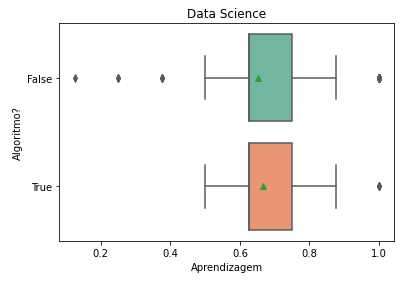
\includegraphics[width=0.45\textwidth]{ds-boxplot-by-algorithm}
	\caption{Distribuição da aprendizagem no cursos de DS para cada sub-conjunto analisado: aulas de algoritmos (\foreign{true} no eixo vertical) e as demais. Os triângulos verdes indicam a média amostral.}
	\label{fig:dist-hipotese-2}
\end{figure}

A figura~\ref{fig:dist-hipotese-2} e a tabela \ref{tab:dist-hipotese-2} apresentam a distribuição da aprendizagem das aulas de ferramentas e das demais do curso de DS.

O curso de DA não tem ênfase em algoritmos.
Por isso não propusemos fazer teste análogo nele.
De fato, podemos verificar no conjunto de dados que a quantidade de aulas com o atributo \foreign{algorithm} = \foreign{true} é zero.

Note, na tabela~\ref{tab:dist-hipotese-2}, que a média amostral das aulas de algoritmo reside no intervalo $[1,1; 1,5]$, que envolve a média amostral das demais aulas.
Além disso, os desvios-padrão são similares.
Isso evidencia que as duas amostras têm origem na mesma população.
Porém, apenas o teste t nos permitirá afirmar.

\begin{table}
	\centering
	\caption{Tamanho da amostra (\#), média (e erro padrão) e desvio-padrão das aulas de algoritmos e demais do curso de DS.}
	\label{tab:dist-hipotese-2}
	\begin{tabular}{lrrr}
		\toprule
		Algoritmo? & \# & $\bar{a}$ & $s_a$ \\
		\midrule
		Sim &  110 &  1,3(2) & 0,88 \\
		Não & 1653 & 1,25(4) & 0,88 \\
		\bottomrule
	\end{tabular}
\end{table}

\begin{table}
	\centering
	\caption{Resultado do teste t no curso de DS}
	\begin{tabular}{lcc}
	\toprule
	Curso & Valor $p$   & Estatística $t$ \\
	\midrule
	DS    & $0,41$      & $0,83$ \\ 
	\bottomrule
	\end{tabular}
\end{table}

Ao efetuarmos o teste de hipótese, obtivemos valor-$p$ de 41\%.
Ou seja, a probabilidade de observarmos a média 1,3(2) numa amostra de uma população com média 1,25(4) é de 41\%, acima do nível de significância de 5\% assumido.
Logo, podemos afirmar que as duas amostras advém da mesma população.
Consequentemente, \emph{não} há diferença de aprendizagem entre as aulas de algoritmos e as demais.
\subsection{Hipótese 3}

Agora voltamos nossa atenção para a possível relação entre a aprendizagem e a satisfação, ritmo e relevância reportados pelos alunos.

O argumento aqui é baseado na aprendizagem individualizada: o ritmo, que pode ser completamente controlado pelo aluno nessa abordagem, oferece vantagem para a aprendizagem.
E como temos informações extras sobre a satisfação e a relevância, vamos considerá-las também como critérios de comparação.

Como a aprendizagem $a$ é uma variável numérica, temos em mãos um problema de regressão.
Argumentamos que uma abordagem classificatória também é possível, desde que se tome o cuidado de garantir a integridade do espaço amostral de $a$, o intervalo $[-4,4]$.
Porém isso ficará para trabalhos futuros.

\begin{figure}[t]
	\centering

	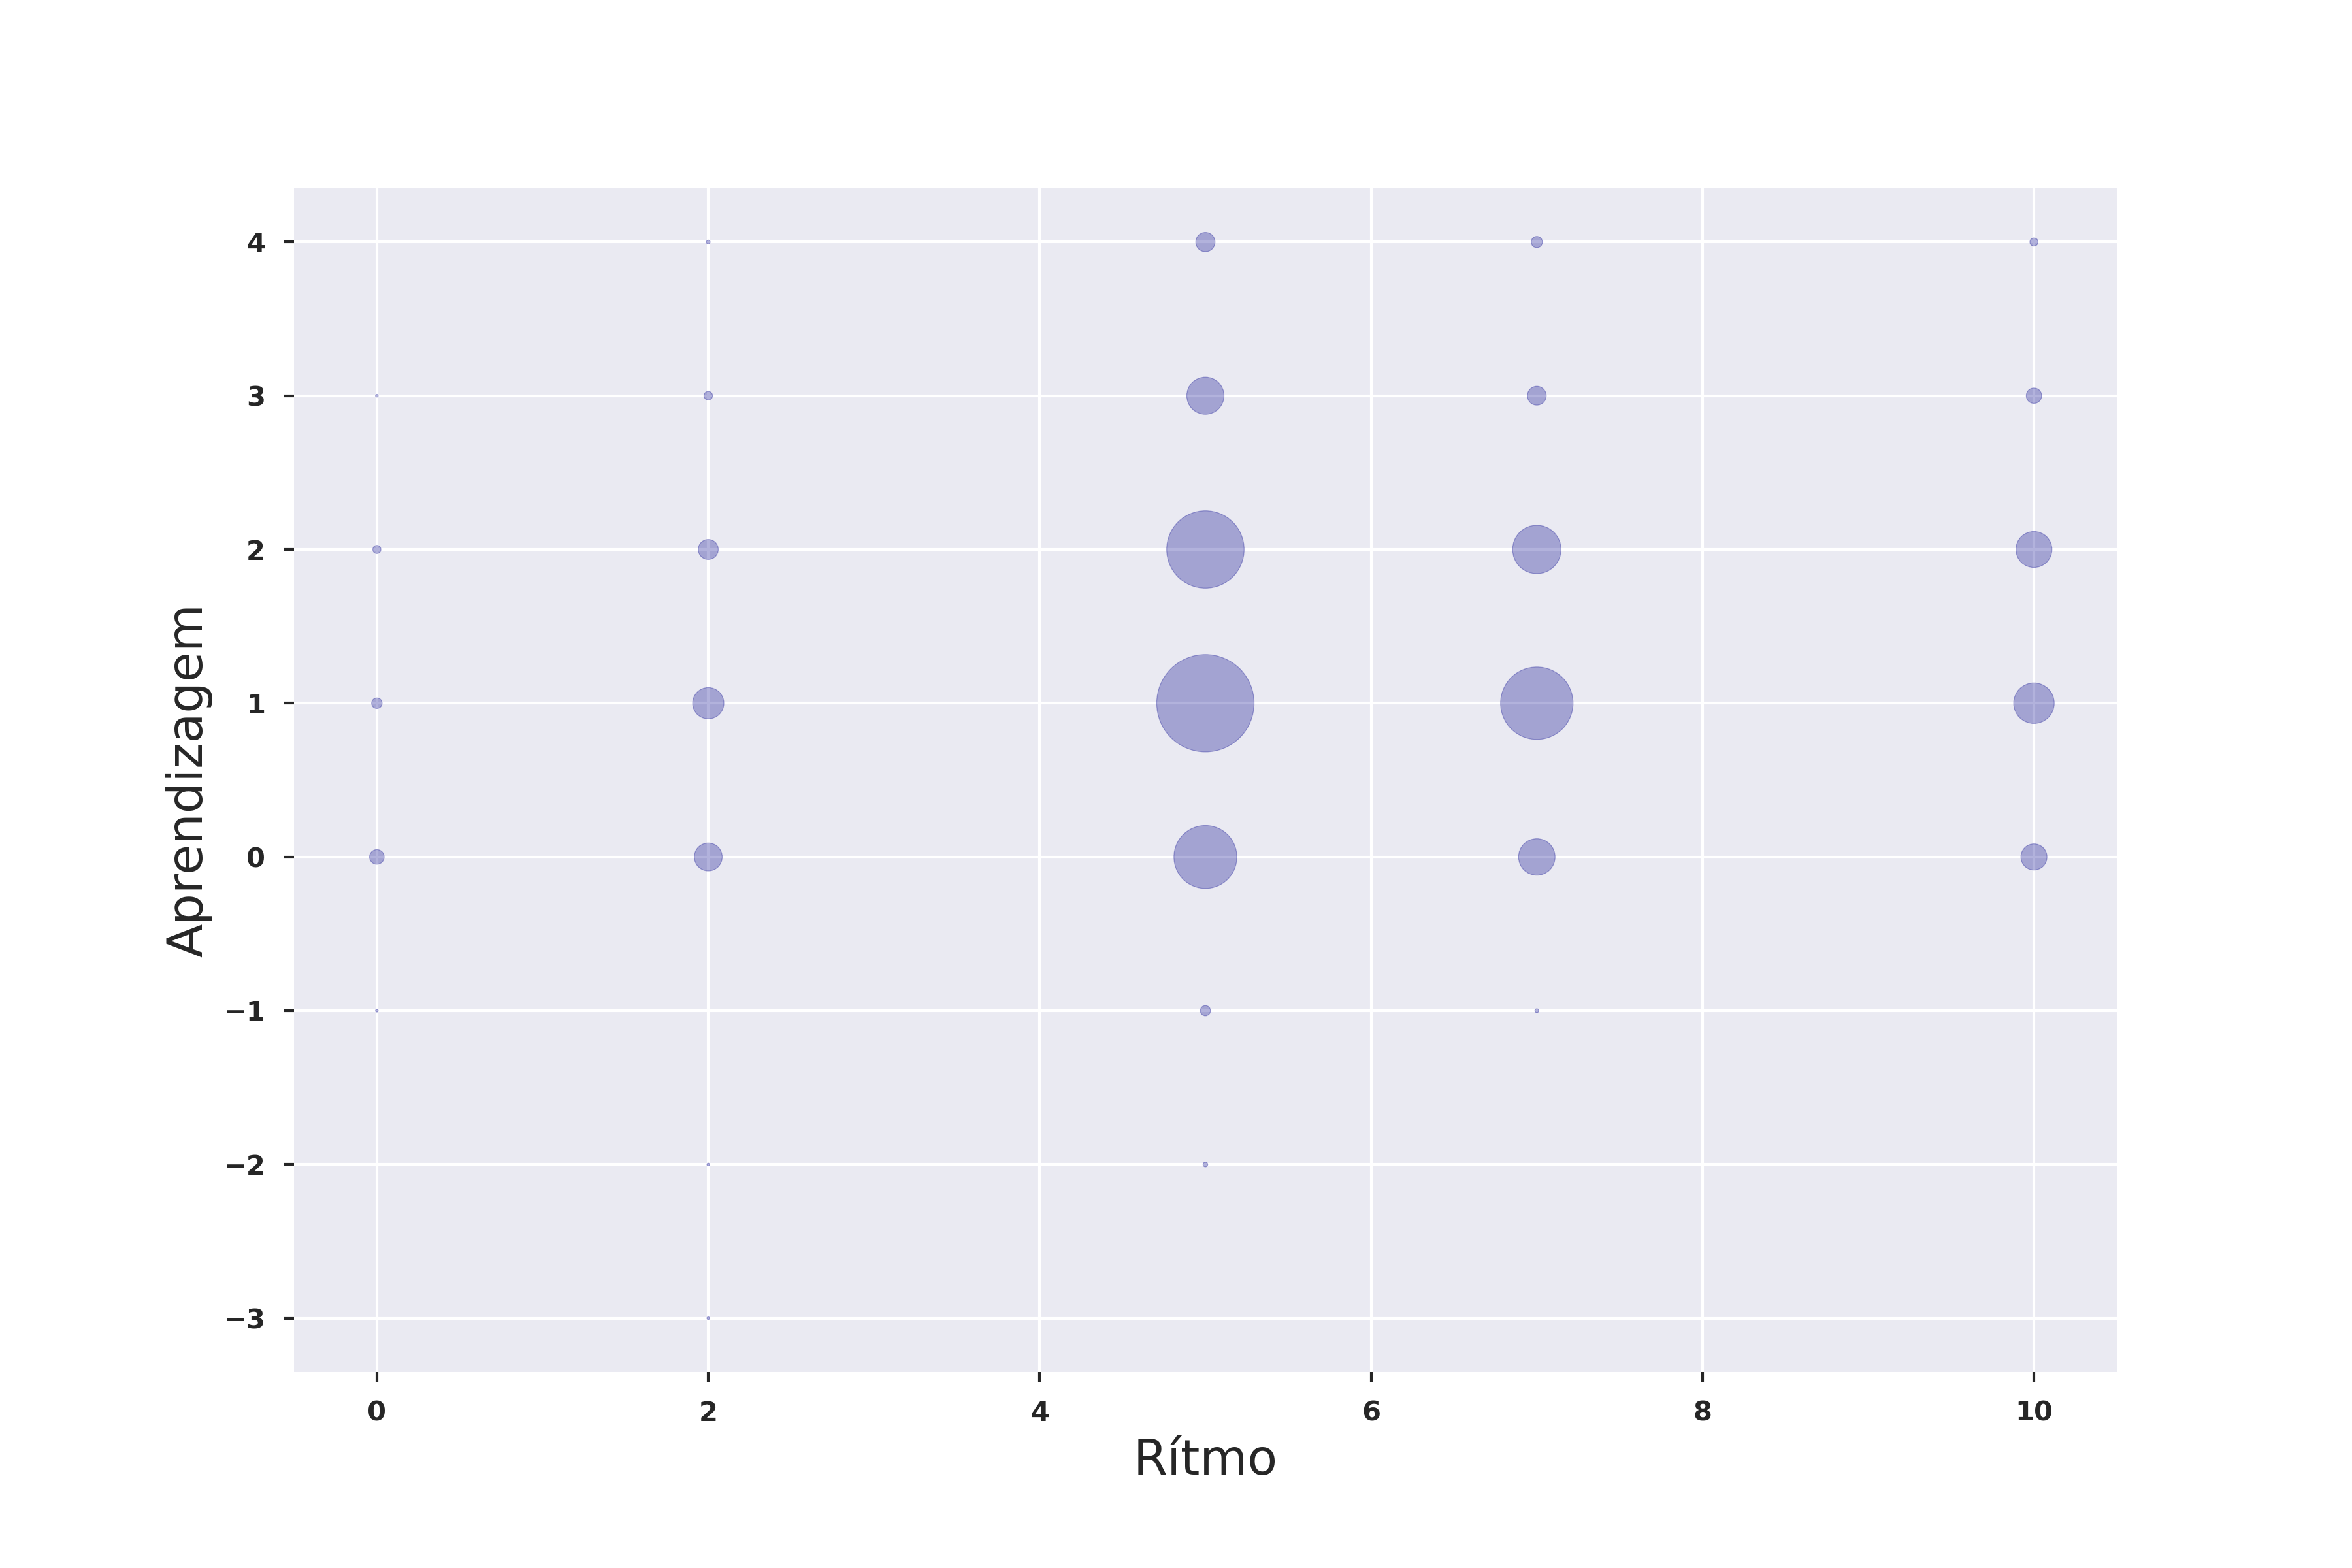
\includegraphics[width=0.5\textwidth]{aprendizagem-vs-ritmo}

	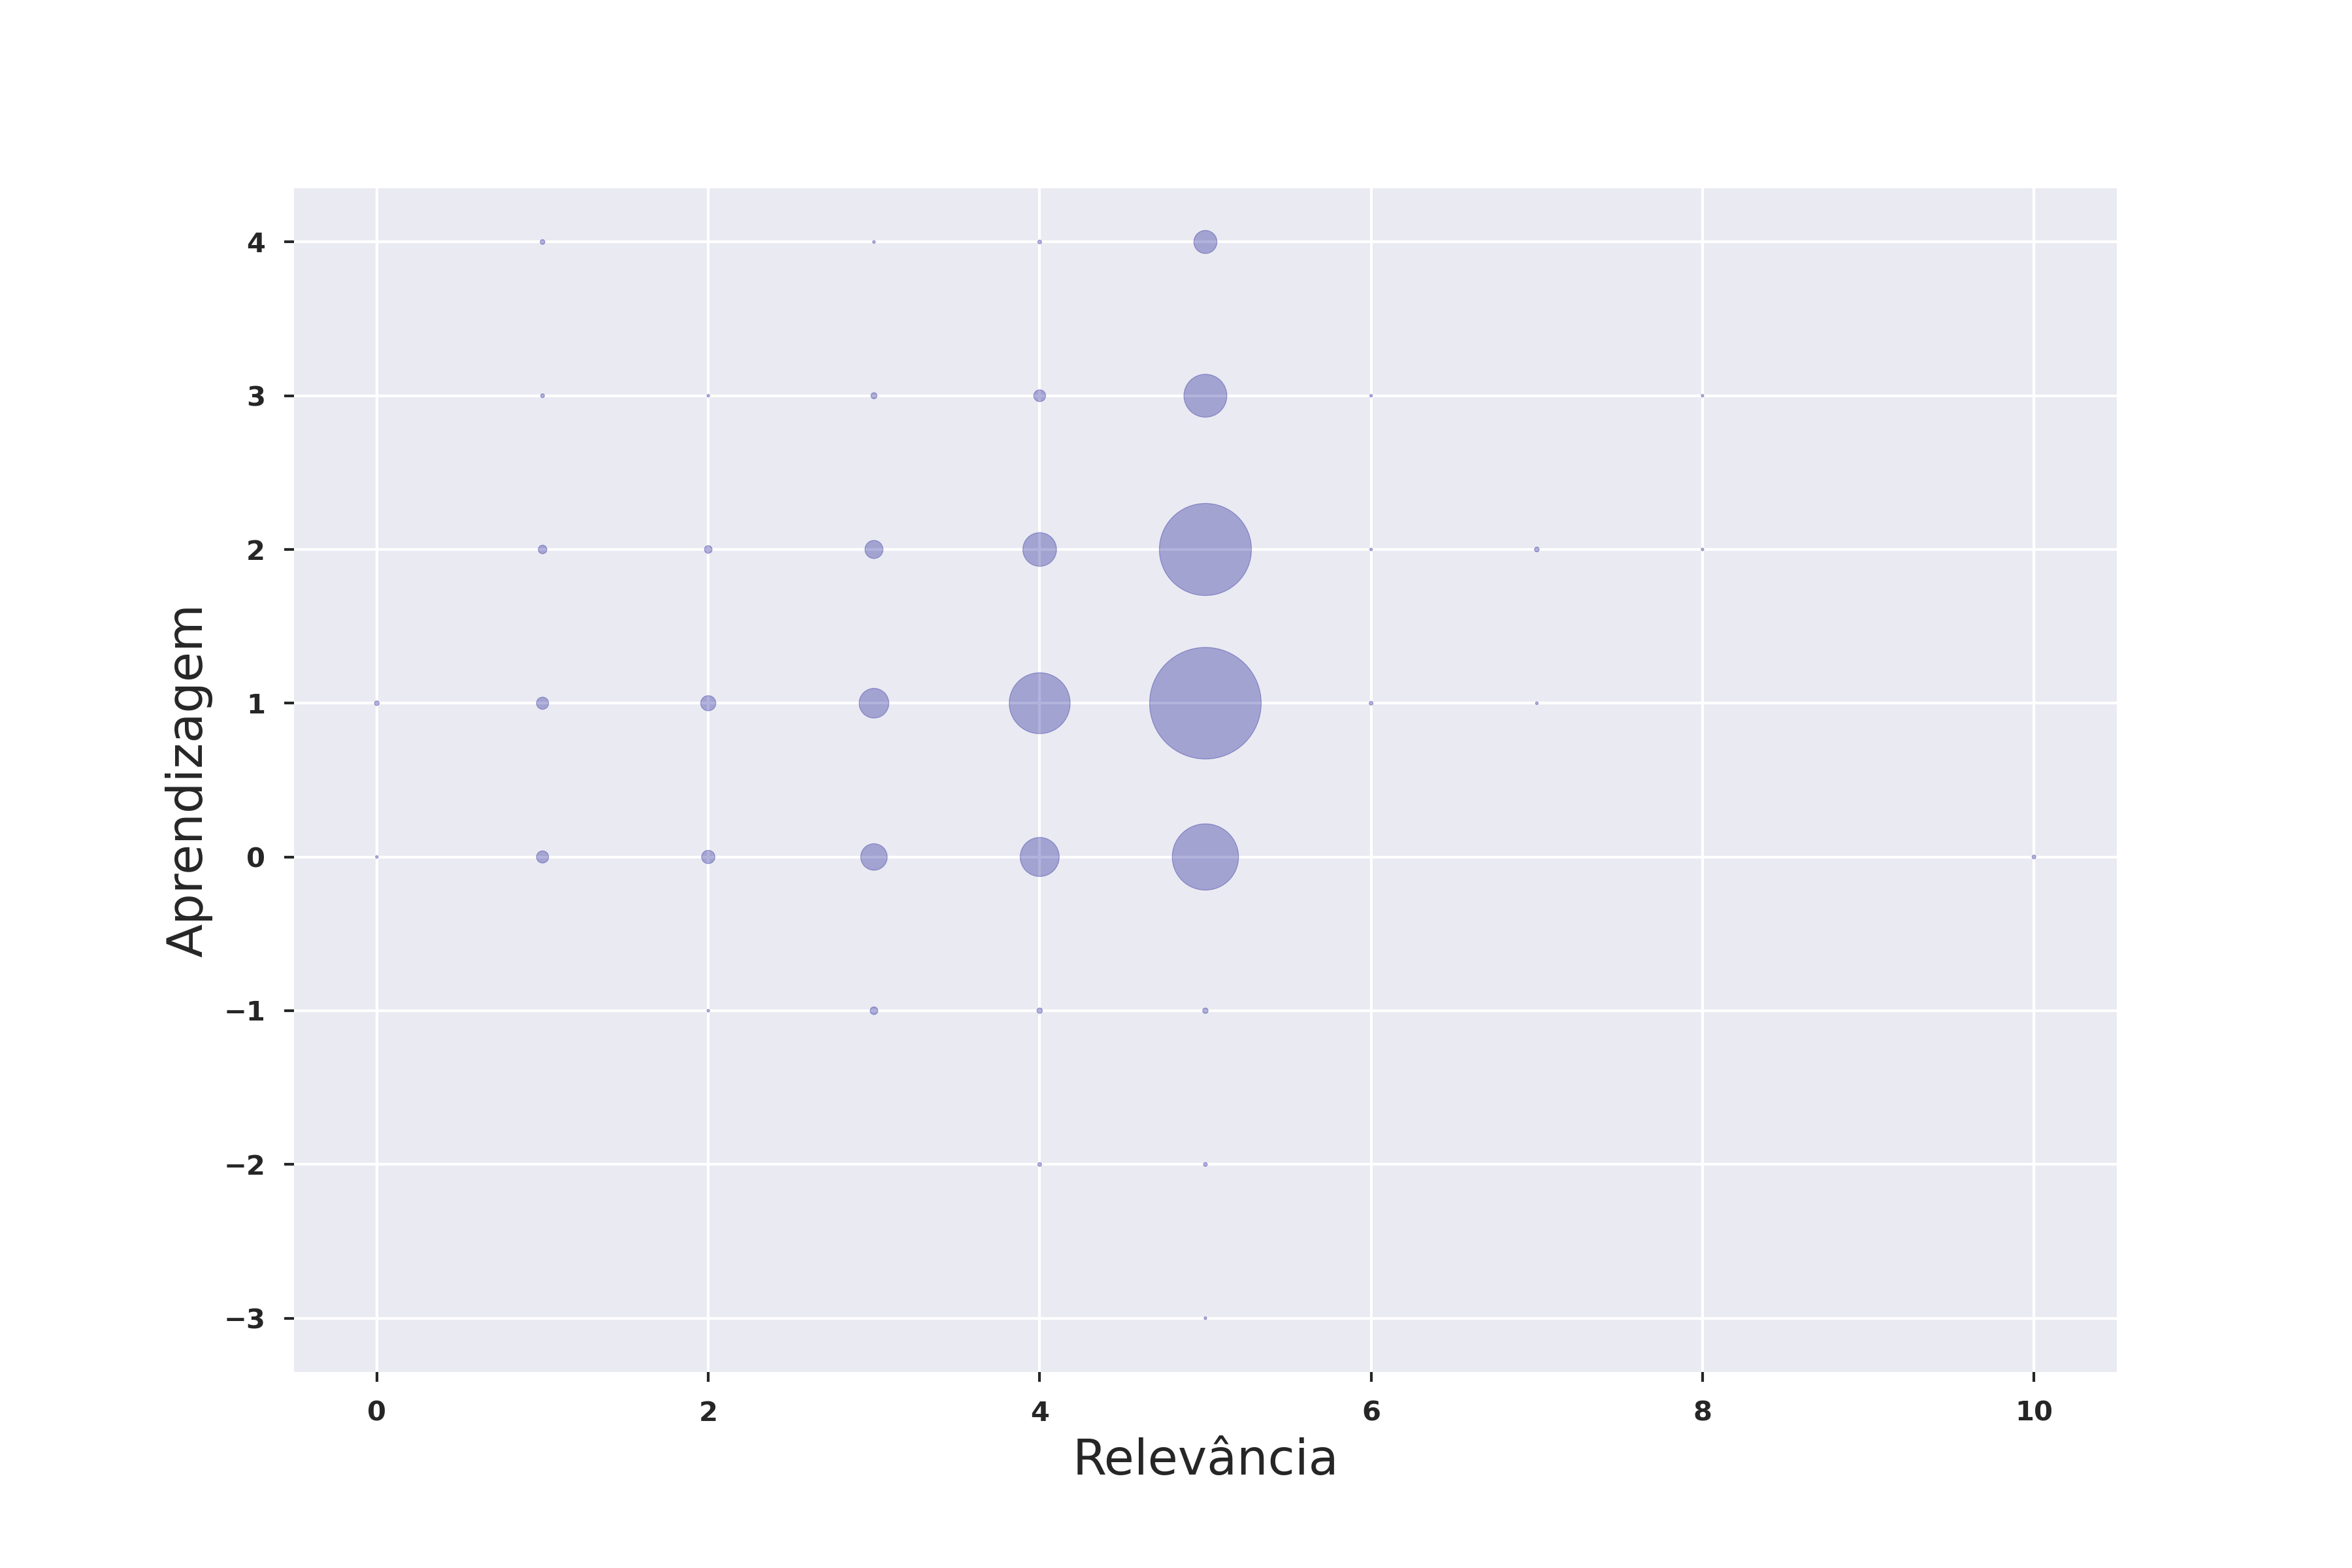
\includegraphics[width=0.5\textwidth]{aprendizagem-vs-relevancia}

	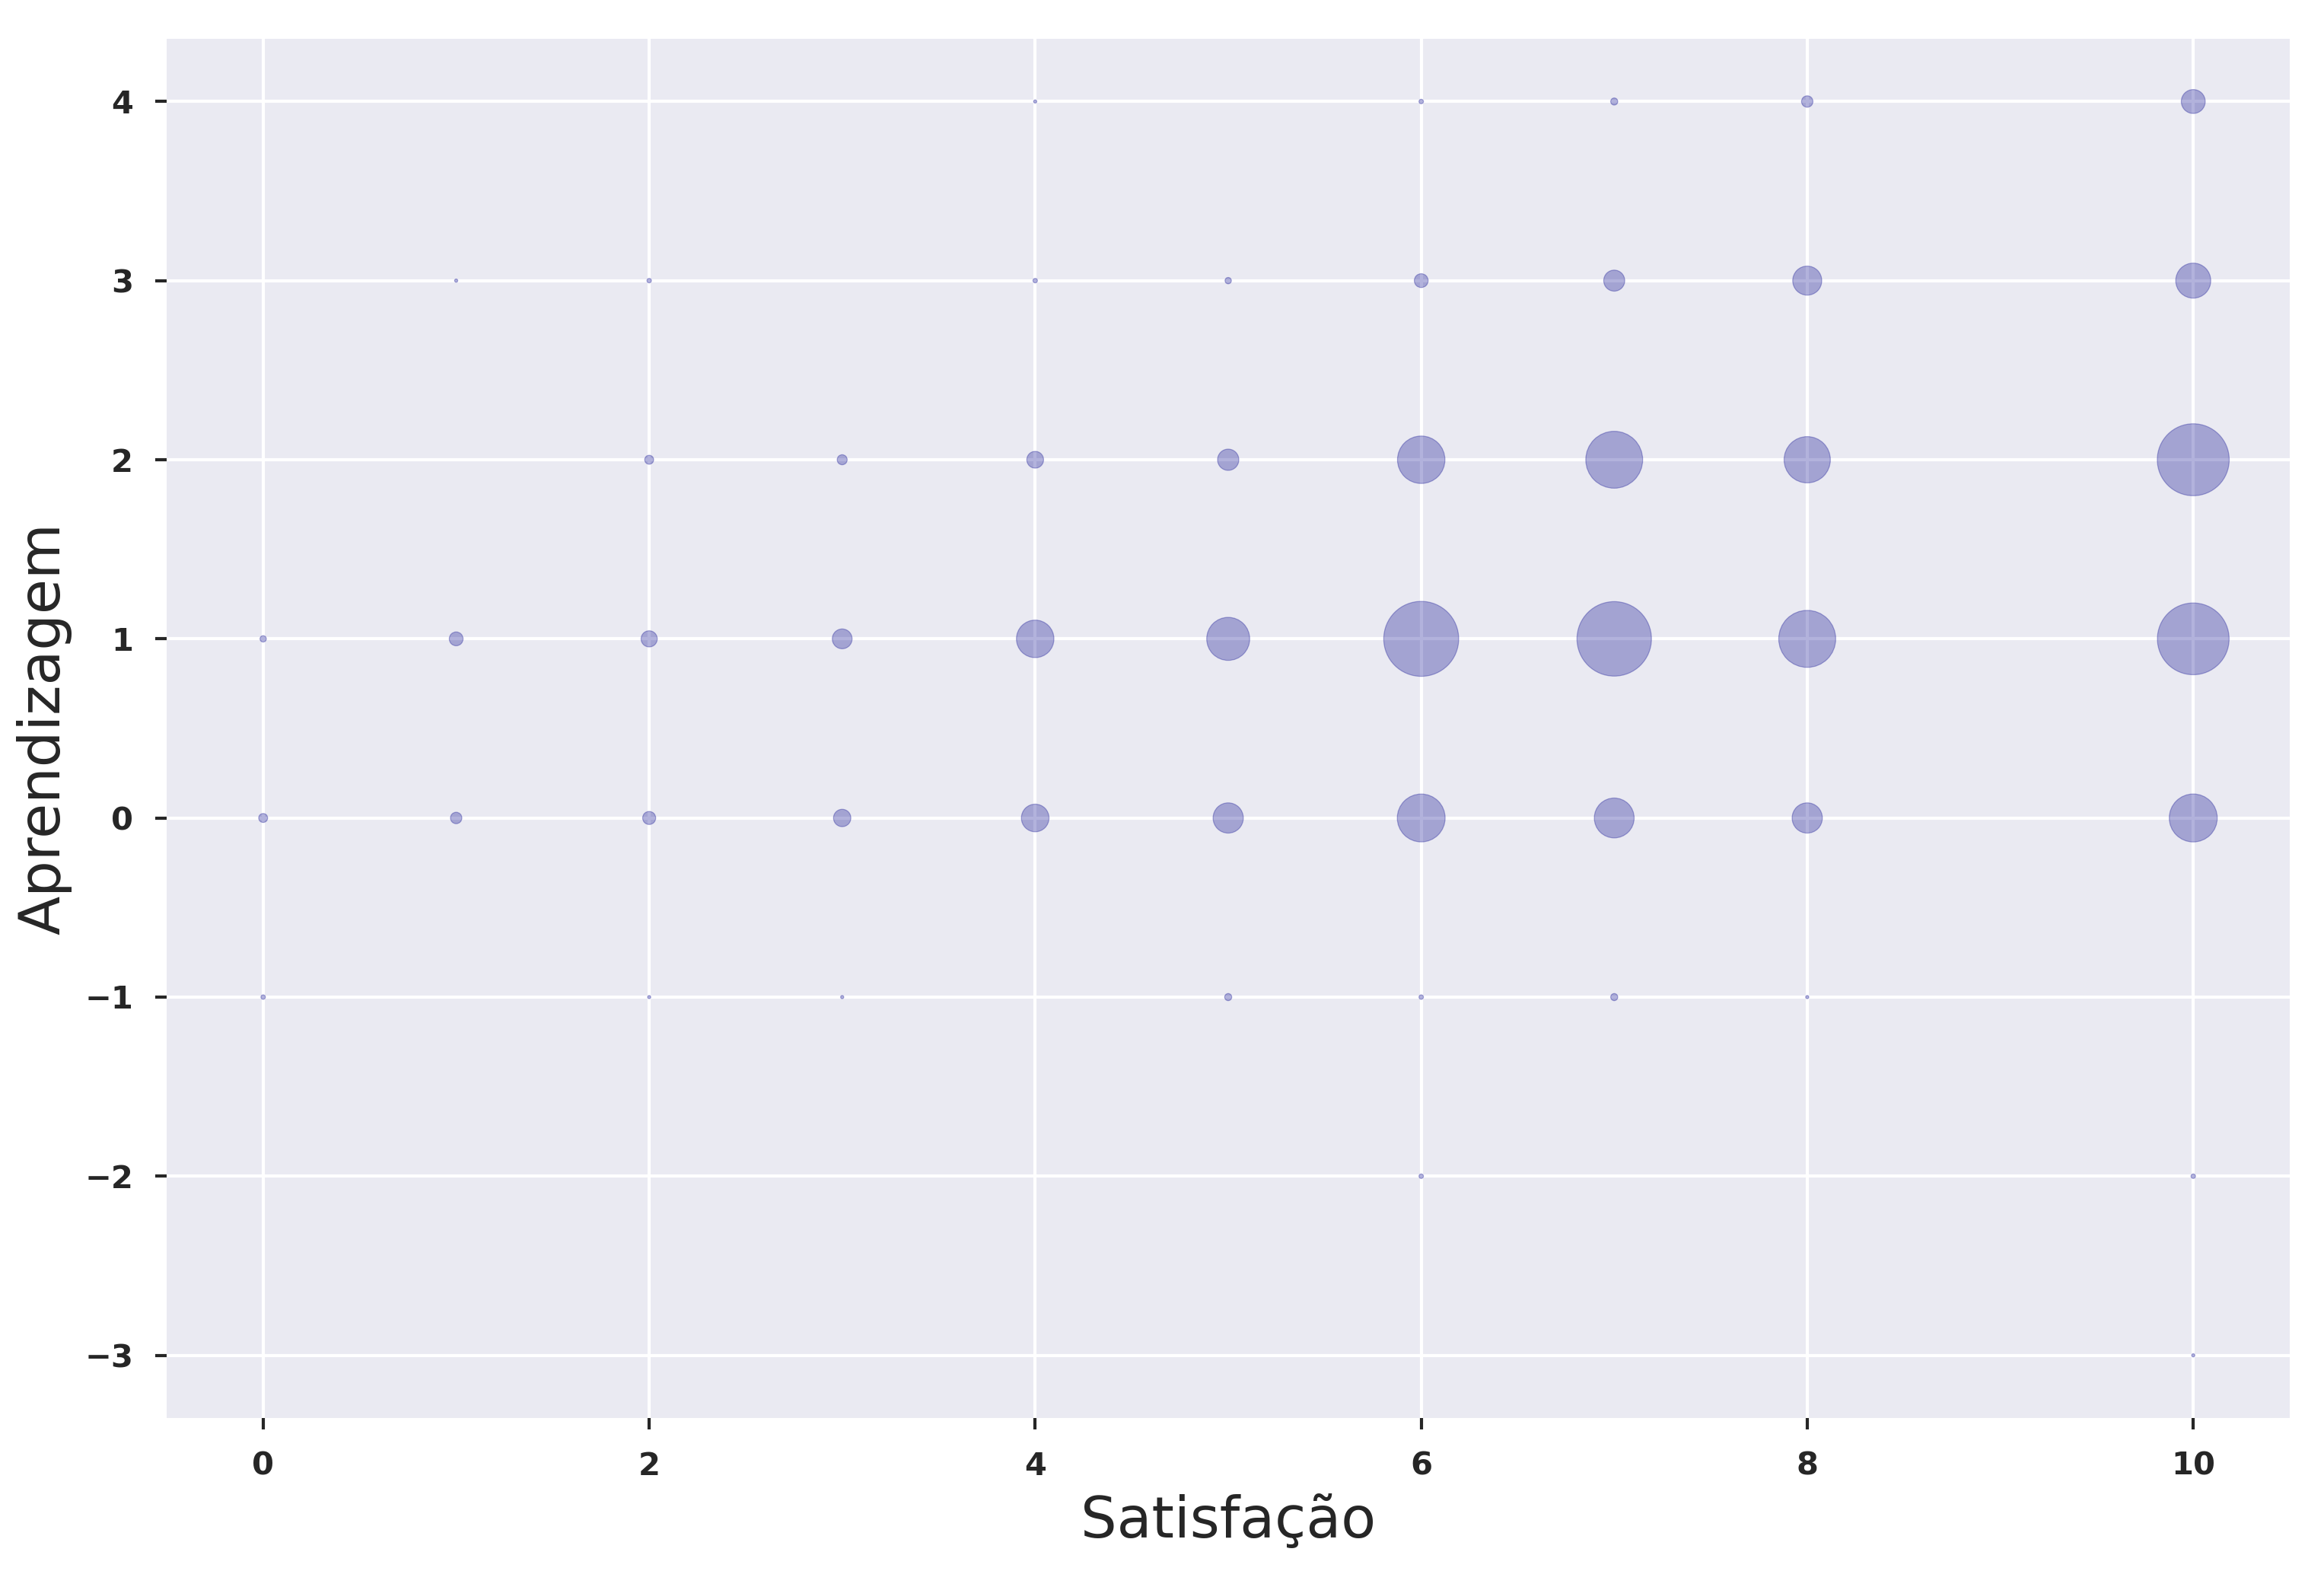
\includegraphics[width=0.5\textwidth]{aprendizagem-vs-satisfacao}

	\caption{\foreign{Bubble-plot} da aprendizagem em função de cada um dos preditores.}
	\label{fig:bubble-plots}
\end{figure}

O modelo de regressão mais simples é o linear.
Porém, uma análise visual dos gráficos de aprendizagem em função de cada um dos preditores não torna evidente qualquer possível relação linear (fig.~\ref{fig:bubble-plots}).
Então experimentamos outros algoritmos de regressão, conforme apresentado na Tabela~\ref{tab:reg-ds-1}.

O conjunto de dados usado para as regressões foi extraído do conjunto completo (Figura~\ref{fig:dataset}), tomando o cuidado de que um dado aluno não estivesse presente mais do que uma vez.
Fizemos esse tratamento com o intuito de evitar correlação entre os exemplos.

Em seguida, aplicamos cada um dos algoritmos a 70\% dos exemplos no conjunto de dados (conjunto de treinamento), explorando sistematicamente o espaço de hiper-parâmetros à procura de um mínimo global no erro quadrático médio da regressão.

O melhor índice de determinação, calculado sobre os 30\% exemplos restantes (conjunto de teste), foi $R^2 \approx 0,193$ para o modelo XGBoost, composto por um conjunto de árvores de decisão simples \cite{Friedman2001}.
Isso significa que nosso melhor modelo é capaz de explicar apenas 19\% das variações na aprendizagem, a partir dos preditores propostos.
Embora seja baixo, podemos argumentar  que a aprendizagem sofre maior influência de outros parâmetros mais importantes, que não temos acesso aqui, como a metodologia de aprendizagem, a qualidade das atividades e conteúdo proposto \etc.

\begin{table}[b]
	\centering
	\caption{Métricas de qualidade dos vários algoritmos de regressão aplicados a DS.}
	\label{tab:reg-ds-1}
	\begin{tabular}{llccc}
		\toprule
		Algoritmo   & Linear? &  RMSE &   MAE & $R^2$\\
		\midrule
		XGBoost  & Não     & 0,769 & 0,581 & \textbf{0,193}\\
		\foreign{Random Forest} & Não & 0,772 & 0,594 & 0,186\\
		Árvore de decisão & Não &  0,775 & 0,596 & 0,181\\
		Adaboost & Não     & 0,806 & 0,629 & 0,113\\
		\foreign{ElasticNet} & Sim & 0,819 & 0,640 & 0,083\\
		SVR & Não & 0,835 & 0,612 & 0,048\\
		\bottomrule
	\end{tabular}
\end{table}

Agora que sabemos que o modelo XGBoost obteve melhor desempenho, podemos experimentar variar os preditores: efetuamos a regressão considerando como preditores as combinações de um, dois e três preditores.
Nesse caso, a métrica mais relevante é o $\bar R^2$, que pondera o índice de determinação pela quantidade de preditores.
Por exemplo, para dois modelos com o mesmo $R^2$, o primeiro com um e o segundo com dois preditores, o melhor modelo é aquele com maior $\bar R^2$.

Os resultados desse experimento estão na Tabela~\ref{tab:r2-adjusted}, ordenados por $R^2$ e $\bar R^2$.
Concluimos que o melhor modelo é de fato o que utiliza todos os três preditores propostos: satisfação, relevância e ritmo.

\begin{table}
	\centering
	\caption{$R^2$ e $\bar R^2$ para o algoritmo XGBoost aplicado a DA e DS.}
	\label{tab:r2-adjusted}
	\begin{tabular}{ccccccc}
		\toprule
		           &            &            & \multicolumn{2}{c}{ Data Science  } & \multicolumn{2}{c}{ Data Analytics }\\
		\midrule
		Relevância & Ritmo      & Satisfação & $R^2$     & $\bar R^2$ & $R^2$     & $\bar R^2$\\
		\midrule
		\checkmark & \checkmark & \checkmark & 0,193 & 0,191 & 0,213 & 0,211 \\
		           & \checkmark & \checkmark & 0,125 & 0,120 & 0,184 & 0,183 \\
		\checkmark &            & \checkmark & 0,115 & 0,114 & 0,147 & 0,146 \\
		           &            & \checkmark & 0,075 & 0,074 & 0,130 & 0,130 \\
		\checkmark & \checkmark &            & 0,071 & 0,070 & 0,096 & 0,095 \\
		\checkmark &            &            & 0,052 & 0,051 & 0,019 & 0,018 \\
		           & \checkmark &            & 0,014 & 0,014 & 0,076 & 0,075 \\
		\bottomrule
	\end{tabular}
\end{table}

A mesma análise pode ser feita para DA, o que nos leva inicialmente à escolha do algoritmo, conforme ilustra a Tabela~\ref{tab:reg-da-1}.
Curiosamente, nesse caso o algoritmo de árvore de decisão obteve melhor desempenho que o \foreign{random forest} (o oposto para DS).
Ainda assim, novamente o melhor (maior $R^2$) algoritmo foi o XGBoost; porém com $R^2$ similar ao caso de DS.

Em seguida variamos os preditores e obtemos os resultados apresentados na Tabela~\ref{tab:r2-adjusted}.
O resultado é similar ao de DS: o modelo que utiliza todos os preditores é melhor.

\begin{table}
	\centering
	\caption{Métricas de qualidade dos vários algoritmos de regressão aplicados a DA.}
	\label{tab:reg-da-1}
	\begin{tabular}{llccc}
		\toprule
		Algoritmo               & Linear? & RMSE  &   MAE & $R^2$\\
		\midrule
		XGBoost                 & Não     & 0,958 & 0,760 & \textbf{0,213}\\
		Árvore de decisão       & Não     & 0,958 & 0,762 & 0,212\\
		\foreign{Random Forest} & Não     & 0,959 & 0,770 & 0,210\\
		Adaboost                & Não     & 0,983 & 0,801 & 0,170\\
		\foreign{ElasticNet}    & Sim     & 0,985 & 0,793 & 0,167\\
		SVR                     & Não     & 0,994 & 0,797 & 0,152\\
		\bottomrule
	\end{tabular}
\end{table}

Resumindo, para DA e DS o melhor modelo XGBoost utilizando os três preditores propostos consegue explicar apenas aproximadamente 20\% das variações observadas (hipótese 3).
Ainda assim, o fato de $R^2$ ser demasiadamente baixo torna essa conclusão duvidosa.



